\section{Durchführung}
\label{sec:Durchführung}

In dem Experiment werden verschiedene Geräte genutzt, um präzise Messergebnisse zu erzielen.
Für die Pumpentechnik wird die Drehschieberpumpe der Firma ILMVAC Typ 300883/AKD16 mit einem Saugvermögen von \(4,6-5,5 \frac{m^3}{h}\)
betrieben. Für die Messungen im Hochvakuum wird mit der Turbomolekularpumpe SST81 von ILMVAC, betrieben bei 1350 Hertz mit
einem Saugvermögen von \(77 \, \frac{L}{s}\) gearbeitet. Bei der Messung der Vakuumwerte kommen zwei verschiedene Messgeräte zum Einsatz:
der kombinierte Pirani/Kaltkathode-Sensor PKR 360 von Pfeiffer Vacuum, ausgelesen mit zwei Anzeigegeräten TPG 361 („SingleGauge“),
sowie der kombinierte Piezo/Pirani-Sensor TPG202 von Pfeiffer Vacuum
\cite{delta_tu_dortmund}.


\begin{figure}
    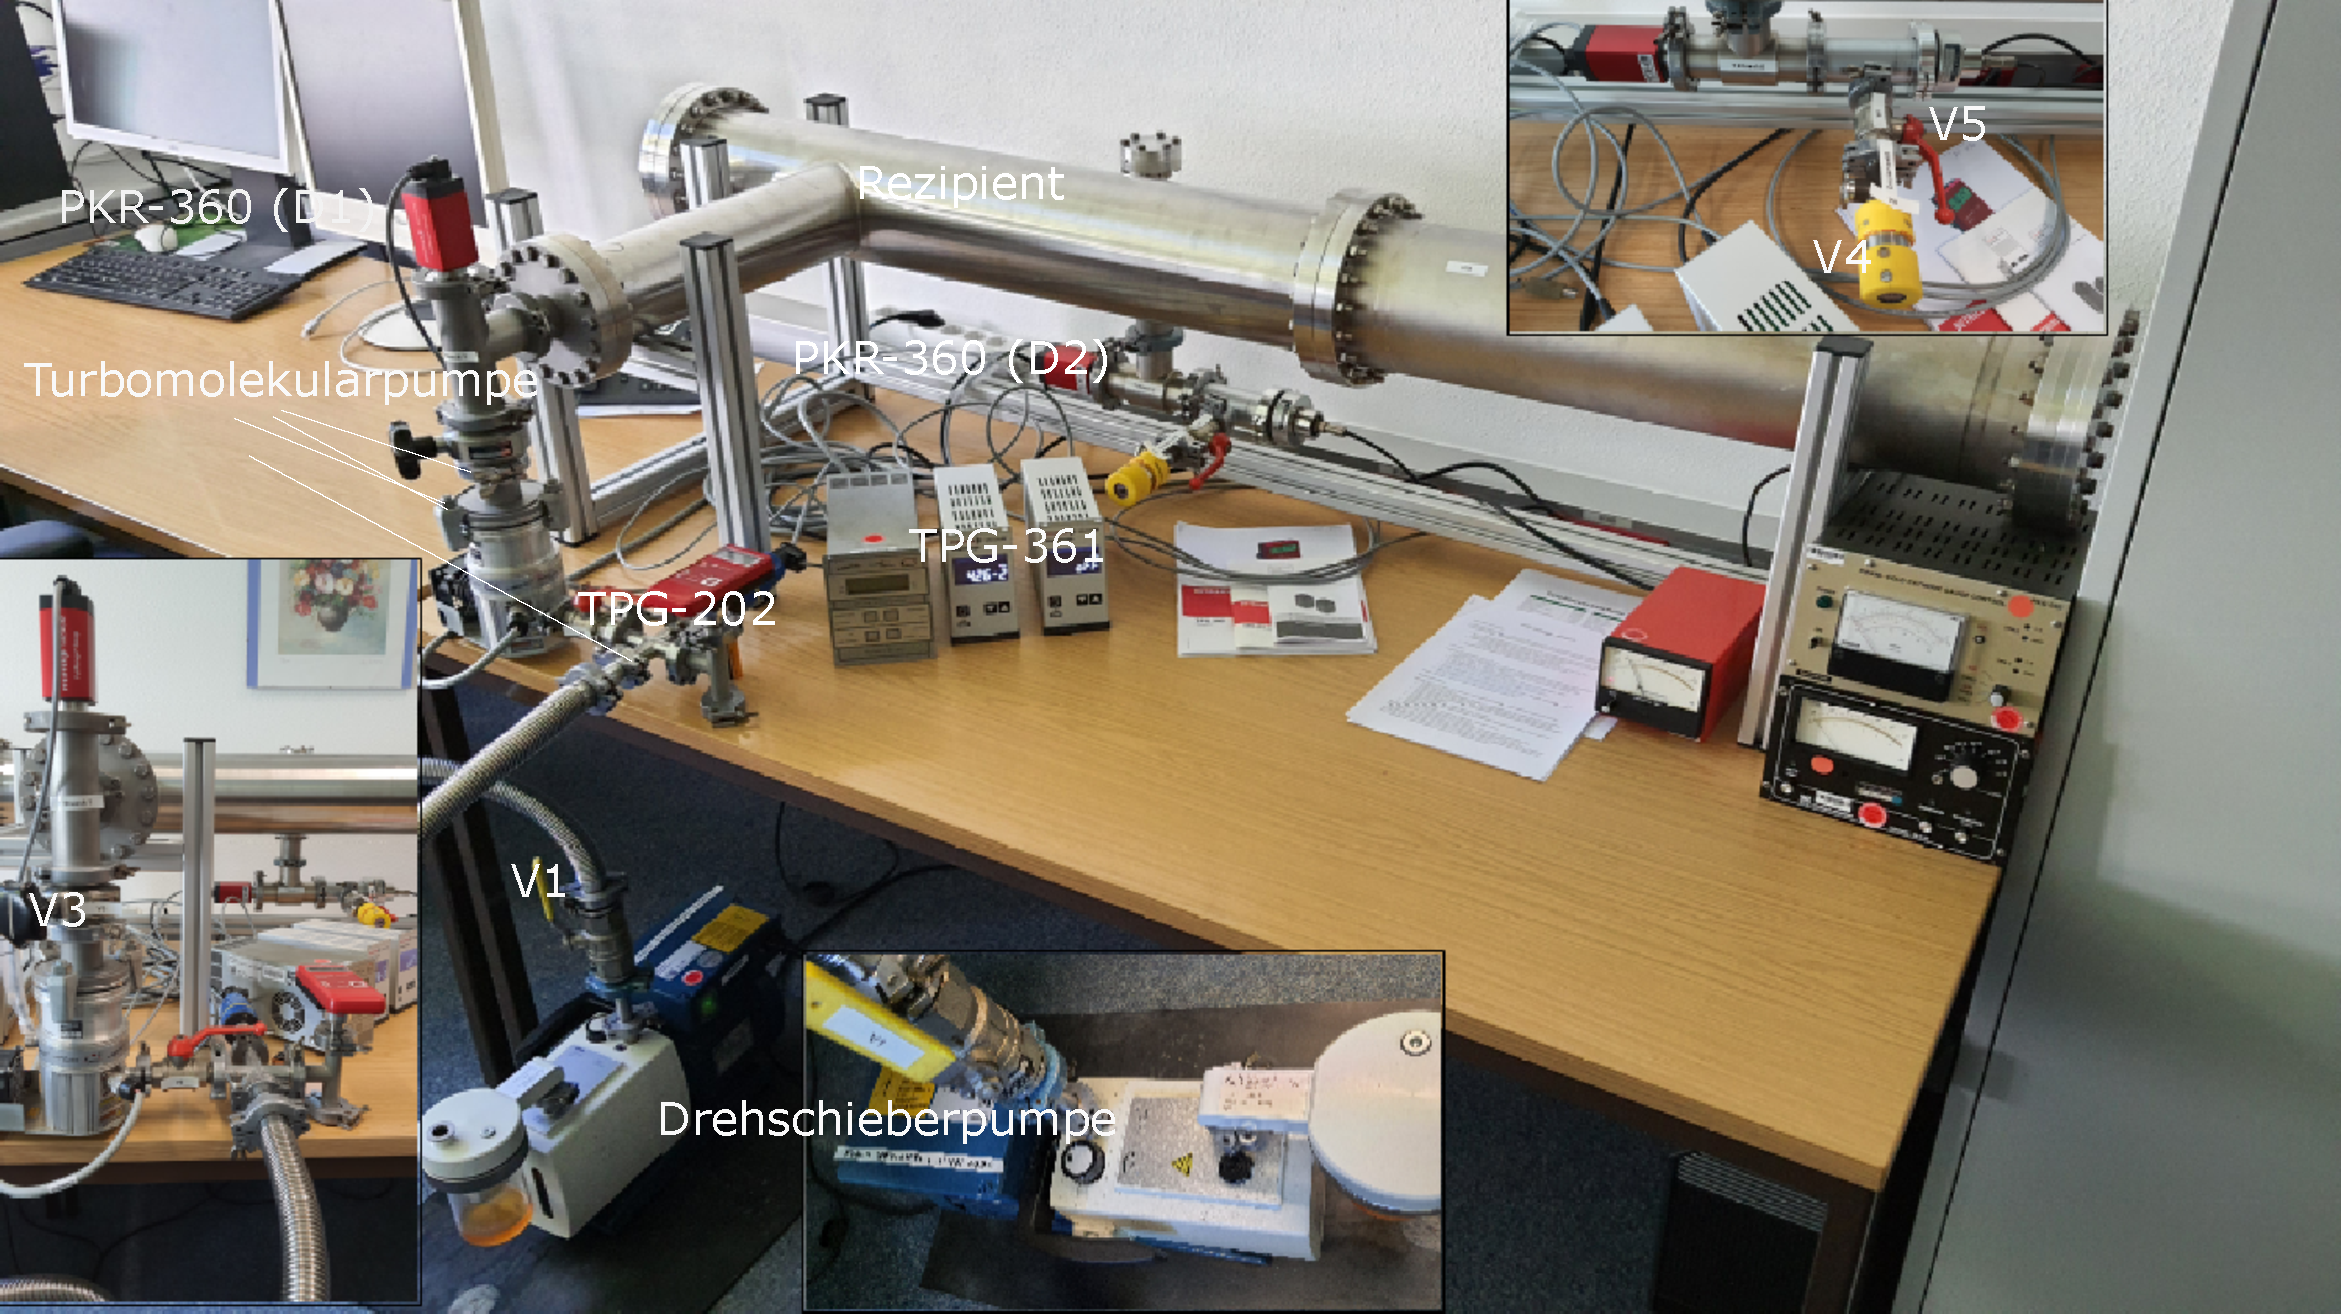
\includegraphics[width=\textwidth]{bilder/versuchsaufbau_anleitung.pdf}
    \caption{Der Versuchsaufbau ohne zusätzliches Rohr. Dieses Rohr würde zwischen der Turbomolekularpumpe und dem Rezipienten verbaut werden.}
\end{figure}


\subsection{Turbomolekularpumpe}
\subsubsection{Evakuierungskurve}


Um die Evakuierungskurve zu bestimmen wird zuerst das schwarze Vential V3 oberhalb der Turbomolekularpumpe geöffnet.
Vorab musste sichergestellt werden, dass bereits Drücke im Bereich des Hochvakuums  von $10^{-7}$ bis $10^{-9}$ bar erreicht wurden.
Die Messwerte werden  mit einem Pirani-Vakuummeter aufgenommen.
Dieses wird in Betrieb genommen, sobald die Turbomolekularpumpe eine Drehzahl von 1350 Hertz erreicht hat.
Um die Kurve zu bestimmen wird das gelbe Dosierventiel auf den Startdruck von $5\cdot10^{-6}$ bar eingestellt während die Turbomolekularpumpe läuft.
Das Kugel- und das Nadelventiel werden dann zeitgleich geschlossen und über einen Zeitraum von 120 Sekunden werden Werte
aufgenommen. Diese werden direkt auf einen angeschlossenen Computer übertragen, abgelesen und gespeichert.
Die Messung wird drei mal durchgeführt, da dies der bestmögliche Kompromiss zwischen Zeitaufwand und Anzahl der Datensätze ist.
Mehr Datensätze würden zu statistisch besseren Ergebnissen führen, passen aber nicht in den Rahmen des Praktikums. 

\subsubsection{Leckratenmessung}
Um die Leckraten zu bestimmen, ist das Ventil V3 geöffnet, mithilfe des Dosierventils V4 werden vier verschiedene 
Gleichgewichtsdrücke eingestellt. Sobald diese eingestellt sind wird das Ventil V3 geschlossen. Die Werte um welche der Druck
im Laufe der Messzeit von 120 Sekunden steigt, werden wieder an den Computer gesendet. Die Gleichgewichtsdrücke sind:
$5\cdot 10^{-8}$ bar, $7\cdot 10^{-8}$ bar, $1\cdot 10^{-7}$ und $2\cdot 10^{-7}$ bar.

\subsubsection{Leckraten mit einem dünnen Verbindungsrohr}
Vor der Turbomolekularpumpe wird für die letzten zwei Messungen ein dünnes Rohr eingebaut. Sobald der Druck wieder Werte erreicht hat in 
welchen die Pumpe arbeiten kann wird jeweils bei $5\cdot 10^{-8}$ bar und bei $2\cdot 10^{-7}$ bar eine weitere Leckratenmessung durchgeführt.


\subsection{Drehschieberpumpe}
\subsubsection{Evakuierungskurve}

Die Bestimmung der Evakuierungskurve der Drehschieberpumpe läuft nach dem selben Prinzip ab. Das gelbe Dosierventil V4 und das Kugelventil V5 werden geöffnet,
und der Rezipient bei abgeklemmter Pumpe (V1 geschlossen) kurz bis zum Atmosphärendruck (ca. 1 bar) belüftet. Die Messung beginnt, sobald die Ventile V4 und V5 wieder geschlossen
sind. Der Druckabfall wird 600 Sekunden lang von einem Computer aufgenommen. Bei diesem Experiment wird ein kombiniertes Piezo-/Pirani-Messgerät
verwendet. Diese Messung findet einmal statt.

\subsubsection{Leckratenmessung}
Um ein Leck zu simulieren wird bei laufender Pumpe mithilfe des Dosierventils V4 ein Gleichgewichtsdruck im Rezipienten eingestellt.
Es werden sechs Messung durchgeführt, jeweils 200 Sekunden lang. Die Messung startet, sobald V1 geschlossen wird. Die dabei eingestellten 
Gleichgewichtsdrücke sind $5\cdot 10^{-4}$ bar, 0,01 bar, 0,05 bar und 0,1 bar. Die Messsung bei 0,1 bar wird dabei dreimal durchgeführt.